\documentclass[aspectratio=169, 10pt]{beamer}

% ==============================================================================
% Packages & Encodings
% ==============================================================================
\usepackage[utf8]{inputenc}
\usepackage[T1]{fontenc}
\usepackage{amsmath, amssymb}
\usepackage{booktabs}
\usepackage{tikz}
\usetikzlibrary{arrows.meta, positioning, shapes.geometric, calc}

% ==============================================================================
% Theme & Color Palette (Clean, Modern, Academic)
% ==============================================================================
\usetheme{Boadilla}
\usecolortheme{default}
\setbeamertemplate{navigation symbols}{} % Remove navigation clutter
\setbeamertemplate{headline}{}

% Custom Colors
\definecolor{PrimaryDark}{RGB}{15, 23, 42}       % Slate 900
\definecolor{AccentBlue}{RGB}{37, 99, 235}       % Blue 600
\definecolor{TealAccent}{RGB}{13, 148, 136}      % Teal 600
\definecolor{CardBg}{RGB}{248, 250, 252}         % Slate 50
\definecolor{CardBorder}{RGB}{226, 232, 240}     % Slate 200
\definecolor{TextDark}{RGB}{30, 41, 59}          % Slate 800
\definecolor{TextMuted}{RGB}{100, 116, 139}      % Slate 500

% Apply Colors to Beamer Elements
\setbeamercolor{title}{fg=PrimaryDark}
\setbeamercolor{frametitle}{fg=PrimaryDark, bg=CardBg}
\setbeamercolor{structure}{fg=AccentBlue}
\setbeamercolor{normal text}{fg=TextDark}
\setbeamercolor{block title}{fg=white, bg=AccentBlue}
\setbeamercolor{block body}{fg=TextDark, bg=CardBg}
\setbeamercolor{block title alerted}{fg=white, bg=TealAccent}
\setbeamercolor{block body alerted}{fg=TextDark, bg=CardBg}

% Frame title styling
\setbeamertemplate{frametitle}{
    \vspace{0.4cm}
    \textbf{\insertframetitle}
    \par\vspace{0.1cm}
    {\color{CardBorder}\hrule height 0.8pt}
}

% Footer
\setbeamertemplate{footline}{
    \leavevmode%
    \hbox{%
        \begin{beamercolorbox}[wd=.6\paperwidth,ht=2.5ex,dp=1.125ex,leftskip=.3cm]{author in head/foot}%
            \color{TextMuted}\footnotesize Intelligent Query Routing Across LLM Ensembles (TREC)
        \end{beamercolorbox}%
        \begin{beamercolorbox}[wd=.4\paperwidth,ht=2.5ex,dp=1.125ex,rightskip=.3cm]{title in head/foot}%
            \color{TextMuted}\footnotesize\hfill Slide \insertframenumber{} of \inserttotalframenumber
        \end{beamercolorbox}%
    }%
    \vskip0pt%
}

% ==============================================================================
% Title Information
% ==============================================================================
\title[\textbf{TREC LLM Routing}]{\LARGE \textbf{Intelligent Query Routing Across LLM Ensembles}}
\subtitle{\large An Information Retrieval Approach to Zero-Inference Model Selection}
\author{\textbf{Course Project Proposal} \\ Information Retrieval}
\institute{TREC Million LLMs Track (NIST)}
\date{\today}

% ==============================================================================
% Document Body
% ==============================================================================
\begin{document}

% ------------------------------------------------------------------------------
% Slide 1: Title Slide
% ------------------------------------------------------------------------------
\begin{frame}[plain]
    \titlepage
\end{frame}

% ------------------------------------------------------------------------------
% Slide 2: Motivation & Problem Statement
% ------------------------------------------------------------------------------
\begin{frame}{1. Motivation \& The Problem Statement}
    \begin{columns}[T]
        \begin{column}{0.5\textwidth}
            \begin{block}{\textbf{The Practical Challenge}}
                \begin{itemize}
                    \item \textbf{Explosion of LLMs:} Today's ecosystem consists of hundreds of specialized models (code, math, medical, reasoning, fast compact models).
                    \item \textbf{The Inefficiency Dilemma:} 
                    \begin{itemize}
                        \item Sending all prompts to massive models is \textbf{costly and slow}.
                        \item Querying multiple models simultaneously is \textbf{wasteful}.
                    \end{itemize}
                \end{itemize}
            \end{block}
        \end{column}

        \begin{column}{0.5\textwidth}
            \begin{alertblock}{\textbf{The Core Research Question}}
                \textit{"Given a user prompt and a large pool of $N$ LLMs, can we predict and rank which model will provide the highest-quality answer \textbf{without executing the models at test time}?"}
            \end{alertblock}
            
            \vspace{0.3cm}
            \textbf{Key Constraint:} 
            \begin{itemize}
                \item \textbf{Zero Test-Time Inference:} Routing must rely purely on precomputed offline capabilities, metadata, and past performance signatures.
            \end{itemize}
        \end{column}
    \end{columns}
\end{frame}

% ------------------------------------------------------------------------------
% Slide 3: Dataset & Benchmark
% ------------------------------------------------------------------------------
\begin{frame}{2. Benchmark Dataset: TREC Million LLMs Track}
    \begin{columns}[T]
        \begin{column}{0.48\textwidth}
            \begin{block}{\textbf{The Benchmark}}
                \begin{itemize}
                    \item Organized by \textbf{NIST (TREC)}, standardizing LLM evaluation and routing across large model pools.
                    \item Involves \textbf{150 distinct LLMs} ranging from small open-weights to proprietary APIs.
                \end{itemize}
            \end{block}
            
            \vspace{0.2cm}
            \begin{block}{\textbf{Discovery Data (Offline Knowledge)}}
                \begin{itemize}
                    \item Historical queries and model responses.
                    \item \textbf{Token Log-Probabilities:} Intrinsic model confidence / uncertainty profiles for each past response.
                \end{itemize}
            \end{block}
        \end{column}

        \begin{column}{0.48\textwidth}
            \begin{alertblock}{\textbf{Development Set \& Ground Truth}}
                \begin{itemize}
                    \item Thousands of diverse evaluation queries across domains (math, code, open-domain QA).
                    \item \textbf{Relevance Labels (`qrels'):} Graded expertise scores assigned to Query-LLM pairs based on human and automated multi-evaluator benchmarks.
                \end{itemize}
            \end{alertblock}

            \vspace{0.2cm}
            \begin{exampleblock}{\textbf{What We Build From This}}
                \begin{itemize}
                    \item LLM Semantic Profiles (what each model knows).
                    \item Query-Conditioned Uncertainty Signatures.
                \end{itemize}
            \end{exampleblock}
        \end{column}
    \end{columns}
\end{frame}

% ------------------------------------------------------------------------------
% Slide 4: Abstract Methodology (Architecture Diagram)
% ------------------------------------------------------------------------------
\begin{frame}{3. Abstract Methodology: Two-Stage Hybrid L2R Router}
    \vspace{-0.2cm}
    \begin{center}
    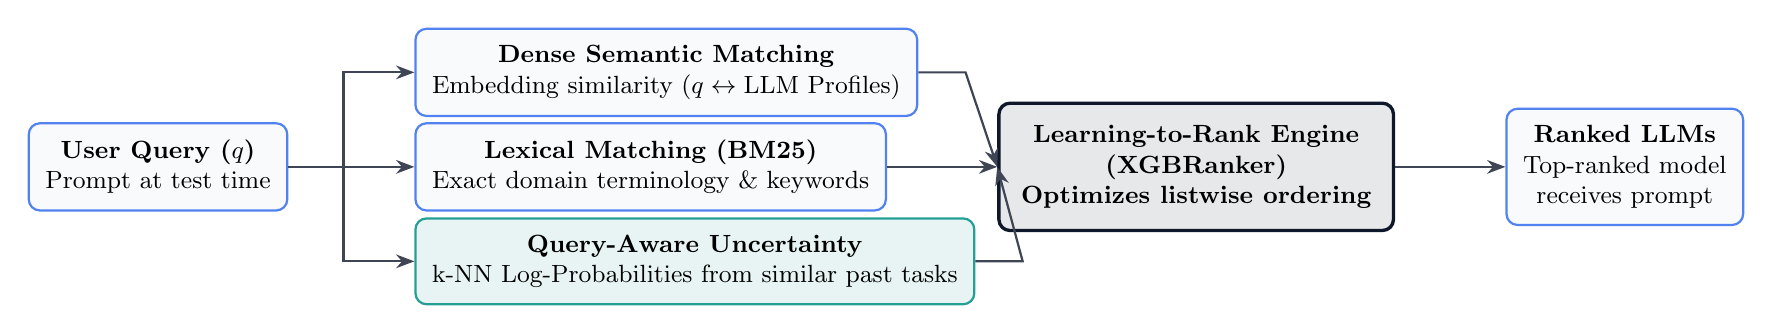
\begin{tikzpicture}[
        node distance=0.85cm and 1.2cm,
        box/.style={draw=AccentBlue!80, fill=CardBg, thick, rounded corners=4pt, align=center, inner sep=6pt, font=\small},
        accentbox/.style={draw=TealAccent!90, fill=TealAccent!10, thick, rounded corners=4pt, align=center, inner sep=6pt, font=\small},
        mainbox/.style={draw=PrimaryDark, fill=PrimaryDark!10, very thick, rounded corners=4pt, align=center, inner sep=8pt, font=\bfseries\small},
        arrow/.style={-{Stealth[scale=1.0]}, thick, color=PrimaryDark!80}
    ]
        % Nodes
        \node[box] (query) {\textbf{User Query ($q$)}\\Prompt at test time};
        
        \node[box, right=1.6cm of query, yshift=1.2cm] (dense) {\textbf{Dense Semantic Matching}\\Embedding similarity ($q \leftrightarrow \text{LLM Profiles}$)};
        \node[box, right=1.6cm of query, yshift=0.0cm] (sparse) {\textbf{Lexical Matching (BM25)}\\Exact domain terminology \& keywords};
        \node[accentbox, right=1.6cm of query, yshift=-1.2cm] (uncertainty) {\textbf{Query-Aware Uncertainty}\\k-NN Log-Probabilities from similar past tasks};

        \node[mainbox, right=1.4cm of sparse] (l2r) {\textbf{Learning-to-Rank Engine}\\\textbf{(XGBRanker)}\\Optimizes listwise ordering};

        \node[box, right=1.4cm of l2r] (output) {\textbf{Ranked LLMs}\\Top-ranked model \\receives prompt};

        % Connectors
        \draw[arrow] (query.east) -- ++(0.7,0) |- (dense.west);
        \draw[arrow] (query.east) -- ++(0.7,0) |- (sparse.west);
        \draw[arrow] (query.east) -- ++(0.7,0) |- (uncertainty.west);

        \draw[arrow] (dense.east) -| ++(0.6,0) -- (l2r.west);
        \draw[arrow] (sparse.east) -- (l2r.west);
        \draw[arrow] (uncertainty.east) -| ++(0.6,0) -- (l2r.west);

        \draw[arrow] (l2r.east) -- (output.west);
    \end{tikzpicture}
    \end{center}

    \vspace{0.1cm}
    \begin{itemize}
        \item \textbf{Stage 1: Multi-Signal Profiling} combines \textit{semantic content}, \textit{lexical keywords}, and \textit{historical model uncertainty}.
        \item \textbf{Stage 2: Learning-to-Rank} learns the non-linear interaction between query type and model strengths.
    \end{itemize}
\end{frame}

% ------------------------------------------------------------------------------
% Slide 5: Evaluation Methodology & Rigor
% ------------------------------------------------------------------------------
\begin{frame}{4. Evaluation Protocol \& Success Metrics}
    \begin{columns}[T]
        \begin{column}{0.5\textwidth}
            \begin{block}{\textbf{Standard IR Ranking Metrics}}
                Evaluated using official TREC tools (\texttt{ir\_measures}):
                \begin{itemize}
                    \item \textbf{nDCG@10 \& nDCG@20:} Measures graded ranking quality (rewarding top placements for the highest-performing models).
                    \item \textbf{MRR (Mean Reciprocal Rank):} Measures how quickly the single best model appears in the ranking.
                \end{itemize}
            \end{block}
            
            \vspace{0.2cm}
            \begin{block}{\textbf{Baseline for Comparison}}
                \begin{itemize}
                    \item \textbf{Standard Dense Bi-Encoder Baseline:} Single-stage cosine similarity using sentence transformers on aggregated past text.
                \end{itemize}
            \end{block}
        \end{column}

        \begin{column}{0.5\textwidth}
            \begin{alertblock}{\textbf{Experimental Rigor: GroupKFold}}
                \begin{itemize}
                    \item \textbf{Zero Leakage:} Validation queries are grouped strictly by \texttt{query\_id}.
                    \item Guarantees that the router is tested on \textbf{completely unseen queries}, reflecting real-world deployment.
                \end{itemize}
            \end{alertblock}

            \vspace{0.2cm}
            \begin{exampleblock}{\textbf{Planned Analysis \& Ablations}}
                \begin{itemize}
                    \item \textbf{Feature Importance:} Value added by uncertainty/LogProb vs.\ text embeddings.
                    \item \textbf{Domain Breakdown:} Performance on coding vs.\ reasoning vs.\ conversational queries.
                \end{itemize}
            \end{exampleblock}
        \end{column}
    \end{columns}
\end{frame}

% ------------------------------------------------------------------------------
% Slide 6: Expected Deliverables & Impact
% ------------------------------------------------------------------------------
\begin{frame}{5. Project Roadmap \& Expected Outcomes}
    \begin{columns}[T]
        \begin{column}{0.55\textwidth}
            \begin{block}{\textbf{Execution Plan}}
                \begin{enumerate}
                    \item \textbf{Baseline Replication:} Establish verified benchmarks using official TREC scripts.
                    \item \textbf{Feature Pipeline:} Extract dense, sparse, and k-NN uncertainty features from discovery metadata.
                    \item \textbf{L2R Model Tuning:} Optimize gradient boosted ranking trees via Bayesian hyperparameter search.
                    \item \textbf{Ablation Study \& Reporting:} Quantify the marginal contribution of each signal.
                \end{enumerate}
            \end{block}
        \end{column}

        \begin{column}{0.45\textwidth}
            \begin{exampleblock}{\textbf{Expected Contributions}}
                \begin{itemize}
                    \item Demonstrating that \textbf{Hybrid L2R + Uncertainty} dramatically outperforms naive dense retrieval.
                    \item \textbf{Production Efficiency:} Sub-15ms routing decision without expensive real-time LLM calls.
                    \item Reproducible code repository, detailed experimental report, and ablation analysis.
                \end{itemize}
            \end{exampleblock}
        \end{column}
    \end{columns}

    \vspace{0.5cm}
    \begin{center}
        \large \textbf{Thank You!} \\
        \normalsize \textit{Questions \& Discussion}
    \end{center}
\end{frame}

\end{document}
